\documentclass[a4paper,12pt]{report}
\usepackage{../courslatex}
\usepackage{theorie}



\renewcommand{\titreChapitre}{Ensembles de nombres et calcul numérique} 
\begin{document}
\chapter{Ensembles de nombres et calcul numérique}
\thispagestyle{fancy}
\section{Les ensembles de nombres}
Voici les ensembles de nombres avec lesquels nous travaillerons cette année. 
\begin{itemize}
	\item $\mathbb{N}$ appelé l'ensemble des entiers est donné par $\mathbb{N}=\{0,1,2,3,\ldots\}$.
	\item $\mathbb{Z}$ appelé l'ensemble des entiers relatifs est donné par $\mathbb{Z}=\{\ldots -3,-2,-1,0,1,2,3,\ldots\}$.
	\item $\mathbb{Q}$ appelé l'ensemble des nombres rationnels est donné par $\mathbb{Q}=\{\frac{p}{q} \mid p,q\in \mathbb{Z} \text{ et } q\neq 0 \}$. 
	
	La barre verticale\,$\mid$ se lit "tel que", ainsi $\mathbb{Q}$ est l'ensemble des fractions $\frac{p}{q}$ telles que $p,q \in \mathbb Z$ et $q\neq 0$.

	On a aussi la caractérisation suivante $\mathbb Q=\{x \mid x \text{ a un développement décimal fini ou infini périodique}\}.$
	\item $\mathbb{R}$ appelé l'ensemble des nombres réels est donné par $\mathbb R=\{x \mid x \text{ a un développement décimal quelconque}\}$.
	On peut également représenter $\mathbb{R}$ comme une droite 
	\begin{center}
	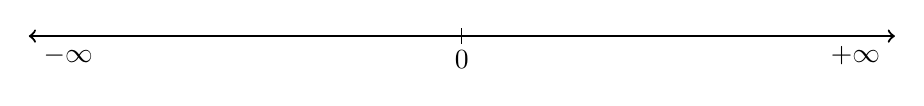
\begin{tikzpicture}
    % Draw the real line
    \draw[thick] (-5,0) -- (5,0); % Adjust the length as needed

    % Add minus infinity symbol on the left
    \node at (-5,0) [below] {$-\infty$};

    % Add plus infinity symbol on the right
    \node at (5,0) [below] {$+\infty$};

    % Add arrowheads to indicate extension to infinity
    \draw[thick,->] (-5,0) -- (-5.5,0);
    \draw[thick,->] (5,0) -- (5.5,0);

    % Optionally, add some tick marks and labels for real numbers
    \foreach \x in {0} {
        \draw (\x,0.1) -- (\x,-0.1); % Tick marks
        \node at (\x, -0.3) {\x}; % Labels for the tick marks
    }
\end{tikzpicture}
\end{center}
\end{itemize}

\begin{defi}[nombre irrationnel]
Un nombre \emph{irrationnel} est un nombre $x\in \R$ tel que $x\not \in \mathbb Q$.
\end{defi}
 Par exemple, $\sqrt{2}, \sqrt{5}$ ou encore $\pi$ sont des nombres irrationnels.

\section{Rappels}
Voici quelques rappels à garder en tête tout au long de l'année. 

\begin{defi}[multiple]
	Un nombre $a\in \N$ est un \emph{multiple} de $b$ s'il existe $n\in \N$ tel que $a=b\cdot n$. 	
\end{defi}

\begin{defi}[diviseur]
	Un nombre $a\in \N$ est un \emph{diviseur} de $b$ s'il existe $n\in \N$ tel que $b: a=n$. 
\end{defi}
Si un $a\in \N$ est un multiple de $b\in \N$, alors $b$ est un diviseur de $a$.

Un procédé qui peut paraître basique, mais qui s'avère fondamental en mahématiques.

\begin{resultat}[division euclidienne]
	Soit $a, b\in \N$. Il existe $q,r\in \N$ vérifiant
	\[a=b\cdot q + r \text{ avec } r<b.\]
	$q$ s'appelle le quotient et $r$ le reste de la division de $a$ par $b$.
\end{resultat}
Derrière ce résultat se cache la division avec des nombres naturels comme vous l'avez apprise à l'école primaire.

Il sera utile de connaître les critères de divisibilité suivants.
Un nombre est divisible par
\begin{enumerate}[leftmargin=2cm]
	\item[{\bfseries deux}] s'il est pair\,;
	\item[{\bfseries trois}] si la somme de ses chiffres est divisible par trois\,;
	\item[{\bfseries quatre}] si le nombre formé par ses deux derniers chiffres est un multiple de quatre\,;
	\item[{\bfseries cinq}] si le chiffre des unités est zéro ou cinq\,;
	\item[{\bfseries neuf}] si la somme de ses chiffres est divisible par neuf.
\end{enumerate}
\begin{defi}[nombre premier]
	\emph{Un nombre premier} est un nombre naturel qui a exactement deux diviseurs.
\end{defi}
On remarque que $1$ n'est pas un nombre premier et que $2$ est le seul nombre premier pair.
Voici la liste des 100 premiers nombres premiers

\begin{quotation}
\noindent$2,\allowbreak\, 3,\allowbreak\, 5,\allowbreak\, 7,\allowbreak\, 11,\allowbreak\, 13,\allowbreak\, 17,\allowbreak\, 19,\allowbreak\, 23,\allowbreak\, 29,\allowbreak\, 31,\allowbreak\, 37,\allowbreak\, 41,\allowbreak\, 43,\allowbreak\, 47,\allowbreak\, 53,\allowbreak\, 59,\allowbreak\, 61,\allowbreak\, 67,\allowbreak\, 71,\allowbreak\, 73,\allowbreak\, 79,\allowbreak\, 83,\allowbreak\, 89,\allowbreak\, 97,\allowbreak\, 101,\allowbreak\, 103,\allowbreak\, 107,\allowbreak\, 109,\allowbreak\, 113,\allowbreak\, 127,\allowbreak\, 131,\allowbreak\, 137,\allowbreak\, 139,\allowbreak\, 149,\allowbreak\, 151,\allowbreak\, 157,\allowbreak\, 163,\allowbreak\, 167,\allowbreak\, 173,\allowbreak\, 179,\allowbreak\, 181,\allowbreak\, 191,\allowbreak\, 193,\allowbreak\, 197,\allowbreak\, 199,\allowbreak\, 211,\allowbreak\, 223,\allowbreak\, 227,\allowbreak\, 229,\allowbreak\, 233,\allowbreak\, 239,\allowbreak\, 241,\allowbreak\, 251,\allowbreak\, 257,\allowbreak\, 263,\allowbreak\, 269,\allowbreak\, 271,\allowbreak\, 277,\allowbreak\, 281,\allowbreak\, 283,\allowbreak\, 293,\allowbreak\, 307,\allowbreak\, 311,\allowbreak\, 313,\allowbreak\, 317,\allowbreak\, 331,\allowbreak\, 337,\allowbreak\, 347,\allowbreak\, 349,\allowbreak\, 353,\allowbreak\, 359,\allowbreak\, 367,\allowbreak\, 373,\allowbreak\, 379,\allowbreak\, 383,\allowbreak\, 389,\allowbreak\, 397,\allowbreak\, 401,\allowbreak\, 409,\allowbreak\, 419,\allowbreak\, 421,\allowbreak\, 431,\allowbreak\, 433,\allowbreak\, 439,\allowbreak\, 443,\allowbreak\, 449,\allowbreak\, 457,\allowbreak\, 461,\allowbreak\, 463,\allowbreak\, 467,\allowbreak\, 479,\allowbreak\, 487,\allowbreak\, 491,\allowbreak\, 499,\allowbreak\, 503,\allowbreak\, 509,\allowbreak\, 521,\allowbreak\, 523,\allowbreak\, 541.$
\end{quotation}

Les nombres premiers sont cruciaux en mathématiques, car ils constituent les briques élémentaires qui permettent de construire tous les autres nombres...

\begin{resultat}[décomposition en produit de nombres premiers]
	Tout nombre entier naturel se décompose de manière unique comme un produit de nombres premiers.
\end{resultat}
\begin{technique}
	Pour décomposer un nombre en produit de nombres premiers, on utilise les critères de divisibilité et les tables de multiplication.
	Par exemple~: 
	\[
  \begin{array}{|l}
    \llap{462~~} 2 \\
    \llap{231~~} 3  \\
    \llap{77~~~} 7  \\
    \llap{11~~~} 11  \\
    \llap{1~~~}    \\ 
  \end{array}
\]
\end{technique}
Voici un résultat fondamental dont la preuve apparaît dans les Élements d'Euclide (Livre 9, Proposition 20).
\begin{resultat}(infinité de nombres premiers)
	Il y a une infinité de nombres premiers.
\end{resultat}
\begin{proof}
	Soit une liste finie de nombres premiers que l'on note $\{p_1,p_2,\ldots,p_k\}$.
	On considère 
	$q=p_1 \cdot p_2 \cdots p_k+1$ le produit de tous ces nombres auquel on ajoute $1$.
	Aucun des nombres $p_1,p_2,\ldots,p_k$ ne divise $q$, car la division euclidienne de $q$ par un de ces nombres donne un reste de $1$.
	Par le théorème de décomposition en nombres premiers, il existe au moins un autre nombre premier en dehors de cette liste et donc l'ensemble des nombres premiers n'est pas fini (on peut toujours s'assurer qu'il en existe un de plus).    
\end{proof}
De grands problèmes de mathématiques encore ouverts (sans réponse) aujourd'hui concernent les nombres premiers.
Des mathématiciens et mathématiciennes passent leur vie à essayer de répondre à ces questions. Voici deux exemples de conjectures. 

La conjecture de Goldbach qui a été formulée en 1742 dans une correspondance avec le mathématicien suisse Euler. 
\begin{quotation}
	Tout nombre entier pair supérieur à 3 peut s'écrire comme une somme de deux nombres premiers.
\end{quotation}

On appelle deux nombres premiers des nombres premiers jumeaux si $p$ et $p+2$ sont premiers.
Par exemple, les nombres $3$ et $5$, $11$ et $13$ ou encore $41$ et $43$. La conjecture est la suivante
\begin{quotation}
	Il existe une infinité de nombres premiers jumeaux.
\end{quotation}
La liste des nombres premiers peut vous aider à déterminer d'autres nombres premiers jumeaux. 

\section{Écriture décimale et fractionnaire}
Un nombre rationnel peut s'écrire sous forme fractionnaire ou sous forme décimale avec développement fini ou infini périodique. 
\begin{technique}[écriture fractionnaire vers décimale]
	Afin de passer de l'écriture fractionnaire à l'écriture décimale, on effectue la division du numérateur par le dénominateur de la fraction.
	On continue jusqu'à ce que la division aboutisse ou jusqu'à obtenir une période (c.f. Série 2).  
\end{technique}
\begin{technique}[écriture décimale vers fractionnaire]
	Il y a deux cas à traiter. Si le développement est fini ou infini périodique.
	Si le développement est fini, on multiplie le nombre décimal par une puissance de $10$ jusqu'à obtenir un nombre entier.
	La fraction égale au nombre décimal de départ est le nombre entier obtenu sur la puissance de $10$.
	Par exemple
	\[31,453=\dfrac{31453}{1000}\]
	Si le développement est infini périodique, nous illustrons la méthode à l'aide d'exemples. 

\begin{minipage}[t]{0.25\textwidth}{
\vspace{0pt}
Si $x=0,\overline{34}$.
	\begin{align*}
		x&=0,\overline{34}\\
		x\cdot 10^2&=34,\overline{34}\\
		x\cdot 10^2&=34+x\\
		x\cdot 10^2-x&=34\\
		x\cdot (10^2-1)&=34\\
		x\cdot 99&=34\\
		x&=\dfrac{34}{99}
	\end{align*}
}
\end{minipage}
\hfill
\begin{minipage}[t]{0.3\textwidth}{
\vspace{0pt}
Si $x=2,\overline{7}$, on écrit $x=2+y$ avec $y=0,\overline{7}$.
	\begin{align*}
		y&=0,\overline{7}\\
		y\cdot 10&=7,\overline{7}\\
		y\cdot 10&=7+y\\
		y\cdot 10-y&=7\\
		y\cdot 9&=7\\
		y&=\dfrac{7}{9}\\
		x&=2+\dfrac{7}{9}\\
		x&=\dfrac{25}{9}
	\end{align*}

}
\end{minipage}
\hfill
\begin{minipage}[t]{0.3\textwidth}{
\vspace{0pt}
Si $x=23,45\overline{678}$, on écrit \[x\cdot 100=2345+0,\overline{678}\] et on pose $y=0,\overline{678}$. 
\begin{align*}
	y&=0,\overline{678}\\
	y\cdot 10^3&=678,\overline{678}\\
	y\cdot 10^3&=678+y\\
	y\cdot 10^3-y&=678\\
	y\cdot 999&=678\\
	y&=\dfrac{678}{999}\\
	x\cdot 100&=2345+\dfrac{678}{999}\\
	x\cdot 100&=\dfrac{2342655}{999}+\dfrac{678}{999}\\
	x\cdot 100&=\dfrac{2343333}{999}\\
	x&=\dfrac{2343333}{99900}\\
x&=\dfrac{781111}{33300}
\end{align*}
}
\end{minipage}
\end{technique}


\section{Puissances}
Voici quelques rappels sur les puissances. 

\begin{defi}(puissance, base, exposant)
	On note $a^n$ le produit répété $n$-fois de $a$ avec lui-même.
	On lit cette expression \enquote{\emph{$a$ à la puissance $n$}}. 
	\[a^n=\underbrace{a\cdot a\cdots a}_{n\text{-fois}}\]
	On appelle $a$ la base et $n$ l'exposant. 
\end{defi}

\begin{proprietes}
	Pour $a,b\in \R$ et $m,n\in \Q$
	\begin{center}

	\begin{inlineumerate}[label={\arabic*)}]
		\item $a^n\cdot b^n=(ab)^n$
		\item $a^m\cdot a^n$=$a^{n+m}$
		\item $\dfrac{a^n}{a^m}=a^{n-m}$ pour $a\neq 0$
		\item $(a^n)^m=a^{n^m}=a^{nm}$
	\end{inlineumerate}
	\end{center}
\end{proprietes}
Rappelons que $a^0=1$ et $0^n=0$ pour tout $n\in \N$. 

\begin{defi}(notation scientifique)
	Un nombre $a\in \Q, a>0$ est en \emph{notation scientifique} s'il est écrit sous la forme 
	\[a=b\cdot 10^n \text{ avec } 1\leq b<10 \text{ et } n\in \Z\]
\end{defi}
\begin{technique}
	La notation scientifique facilite le calcul avec les nombres décimaux.
\end{technique}
\section{Racines}
\begin{defi}(racine carrée)
	\emph{La racine carrée} d'un nombre $a\in \R$ {\bfseries positif} est l'unique nombre {\bfseries positif} $b\in \R$ tel que $b^2=a$. On note $\sqrt[2]{a}=\sqrt{a}=b$. 
\end{defi}
\begin{defi}(racine cubique)
	\emph{La racine cubique} d'un nombre $a\in \R$ est l'unique nombre $b\in \R$ tel que $b^3=a$. On note $\sqrt[3]{a}=b$. 
\end{defi}
Rappelons que $\sqrt{-1}$ n'est pas défini, $\sqrt{1}=1, \sqrt{0}=0$ et $\sqrt[3]{-1}=-1$
\begin{proprietes}
Le propriétés suivantes énoncées pour les racines carrées et cubiques. 

\begin{minipage}[t]{0.5\textwidth}{
\vspace{0pt}
\begin{center}
	{\bfseries Racine carrée}
	\begin{enumerate}[label={\arabic*)}]
\item $\sqrt{a}\cdot \sqrt{b}=\sqrt{a\cdot b}$ pour $a,b\in \R$, $a,b\geq 0$
\item $\dfrac{\sqrt{a}}{\sqrt{b}}=\sqrt{\dfrac{a}{b}}$ pour $a,b\in \R$, $a\geq 0$, $b>0$
\item $\sqrt{a^n}=a^{\frac{n}{2}}$ pour $a\in \R$, $a\geq 0$ et $n\in \N$
\item $\sqrt{a^2}=\lvert a\rvert$ pour $a\in \R$
\item $(\sqrt{a})^2=a$ pour $a\in \R$, $a\geq 0$. 
\end{enumerate}
\end{center}

}
\end{minipage}
\begin{minipage}[t]{0.5\textwidth}{
\vspace{0pt}
{\bfseries Racine cubique}
\begin{center}
	\begin{enumerate}[label={\arabic*)}]
		\item $\sqrt[3]{a}\cdot \sqrt[3]{b}=\sqrt[3]{a\cdot b}$ pour $a,b\in \R$
		\item $\dfrac{\sqrt[3]{a}}{\sqrt[3]{b}}=\sqrt[3]{\dfrac{a}{b}}$ pour $a,b\in \R$, $b>0$
		\item $\sqrt[3]{a^n}=a^{\frac{n}{3}}$ pour $a\in \R$, $n\in \N$
		\item $\sqrt[3]{a^3}=a$ pour $a\in \R$
		\item $(\sqrt[3]{a})^3=a$ pour $a\in \R$. 
\end{enumerate}
\end{center}

}
\end{minipage}
\end{proprietes}
\begin{defi}(conjugué)
	Soient $a,b,c\in \R, c\geq 0$, \emph{le conjugué} de $a+b\sqrt{c}$ est $a-b\sqrt{c}$. Il vérifie \[(a+b\sqrt{c})\cdot (a-b\sqrt{c})=a^2-b^2c.\] 
\end{defi}

Voici deux exemples de calculs faisant intervenir ces propriétés.

\[\dfrac{\sqrt{32}}{\sqrt{6}}\stackrel{\text{propriété } 2)}{=}\sqrt{\dfrac{32}{6}}=\sqrt{\dfrac{16}{3}}=\dfrac{\sqrt{16}}{\sqrt{3}}=\dfrac{4}{\sqrt{3}}\stackrel{\text{c.f. convention ci-dessous}}{=}\dfrac{4\sqrt{3}}{3}\]

\[\sqrt{3}(\sqrt{6}+\sqrt{5})=\sqrt{3}\cdot \sqrt{6}+\sqrt{3}\cdot \sqrt{5}=\sqrt{3\cdot 6}+\sqrt{3\cdot 5}=\sqrt{18}+\sqrt{15}\stackrel{\text{c.f. convention ci-dessous}}{=}3\sqrt{2}+\sqrt{15}\] 

{\bfseries On suit deux conventions avec les racines\,:}

\begin{enumerate}[label={\arabic*)}]
	\item Lorsque $c\in \N$, on extrait les carrés sous la racines, c'est-à-dire qu'on écrit une racine $\sqrt{c}=a\cdot \sqrt{b}$ avec $b\in \N$ le plus petit possible. Pour faire cela, on commence par décomposer $c$ en produit de facteurs premiers, puis on utilise la première et la troisième propriété des racines, par exemple
		\[\sqrt{288}=\sqrt{2^5\cdot 3^2}=\sqrt{2\cdot 2^4\cdot 3^2}=\sqrt{2^4}\cdot \sqrt{3^2}\cdot \sqrt{2}=2^2\cdot 3\cdot \sqrt{2}=12\sqrt{2}\]
		On aurait également pu remarquer
		\[\sqrt{288}=\sqrt{2\cdot 144}=\sqrt{2}\cdot \sqrt{144}=12\sqrt{2}\]
	\item On ne laisse pas de racines au dénominateur d'une fraction dans le résultat d'un calcul. Pour supprimer la racine on a les deux techniques suivantes d'amplification de la fraction en question par $1$.
		
		Si le dénominateur contient une racine simple. 
	\[\dfrac{3}{\sqrt{2}}=\dfrac{3}{\sqrt{2}}\cdot 1=\dfrac{3}{\sqrt{2}}\cdot\dfrac{\sqrt{2}}{\sqrt{2}}=\dfrac{3\sqrt{2}}{\sqrt{2}\cdot \sqrt{2}}=\dfrac{3\sqrt{2}}{2}\]
	Si le dénominateur est de la forme $a+b\sqrt{c}$, on utilise le conjugé. On amplifie la fraction par $1=~\dfrac{a-b\sqrt{c}}{a-b\sqrt{c}}$. 
	\[\dfrac{7}{1+\sqrt{5}}=\dfrac{7}{1+\sqrt{5}}\cdot \dfrac{1-\sqrt{5}}{1-\sqrt{5}}=\dfrac{7(1-\sqrt{5})}{(1+\sqrt{5})(1-\sqrt{5})}=\dfrac{7(1-\sqrt{5})}{1-5}=\dfrac{7(1-\sqrt{5})}{-4}=-\dfrac{7(1-\sqrt{5})}{4}\]
\end{enumerate}


\vspace{1cm}
\textLigne{Notes personnelles ou complément}

\end{document}
